\documentclass[10pt,a4paper]{amsart}
\usepackage[margin=19mm]{geometry}
\usepackage{amsmath,amssymb,mathtools}
\usepackage[scr=rsfs,cal=euler]{mathalfa}
\usepackage{xfrac}
\usepackage[unicode,hidelinks,bookmarks=false]{hyperref}
\newcommand{\ie}{i.e.\ }
\newcommand{\cf}{cf.\ }
\newcommand{\resp}{respectively\ }
\newcommand{\Subsection}{\subsection}
\providecommand{\nobreakdash}{\nobreak\hbox{-}}
\setlength{\emergencystretch}{2em}
\multlinegap0pt
\usepackage{tikz}
\usepackage{mathtools}
\usepackage{amssymb}
\usepackage{xcolor}
\usepackage[shortlabels]{enumitem}
\newtheorem{lemma}{Lemma}
\newcommand{\N}{\mathbb{N}}
\newcommand{\R}{\mathbb{R}}
\renewcommand{\geq}{\geqslant}
\renewcommand{\leq}{\leqslant}
\title{An Improved Bipartition Cover Bound for the Multispecies Coalescent Model}
\author{Zachary McNulty\textsuperscript{a}}
\date{Source: arXiv:2604.09509v2 (CC BY 4.0)}
\begin{document}
\maketitle

\noindent\emph{Source and licence.} An Improved Bipartition Cover Bound for the Multispecies Coalescent Model. Version arXiv:2604.09509v2 (CC BY 4.0), distributed by arXiv under the Creative Commons Attribution 4.0 International licence, http://creativecommons.org/licenses/by/4.0/, as recorded in the arXiv licence metadata for this exact version and shown on the abstract page https://arxiv.org/abs/2604.09509v2. Full licence notice: \texttt{licenses/arxiv-2604.09509-CC-BY-4.0.txt}.\par\smallskip

\noindent\textit{Editorial scope.} Counted unit: the article's lemma lem:balanced\_trees\_minimize\_increasing\_convex\_sums (source0.tex lines 1469--1472). The article's complete original proof of it is delivered with it (source0.tex lines 1474--1597, one \texttt{proof} environment of 124 lines). No mathematics is written, repaired or re-derived: the statement and the proof are the article's own lines, in the article's own notation, and no retained line is substituted or re-flowed.  No further source-local context is needed: every cross-reference of every retained line resolves inside the two delivered spans.  Nothing was omitted from any retained span, so the package carries no omission record.  No retained line contains a citation, so the wrapper carries no bibliography and no bibliography entry.  The retained lines contain the article's own diagram code, which the wrapper typesets with the standard tikz packages; no image file is delivered and the package declares no asset dependency.  Editorial formatting only, in addition: an AMS \texttt{amsart} preamble that restates the article's own declarations and macros used by the retained lines, namely the environments \texttt{lemma} on separate counters, together with the standard packages those lines need.  The retained environments print in this document as Lemma 1 in order of appearance, whereas the article prints the same items with the numbering of its own full document.  The complete native source of the article as distributed in the arXiv e-print for this exact version is bundled unchanged as \texttt{sources/198214/source0.tex}.
\begin{lemma}
 Suppose $\{\alpha_{i}\}_{i=1}^{2k-2}$ are the descendant counts of our rooted binary tree $T$ corresponding to \textit{all} the edges of our tree (not just ones corresponding to nontrivial bipartitions). Moreover, suppose $f: \N \to \R$ is nondecreasing and convex. Then $\sum_i f(\alpha_{i})$ is minimized when $T$ is the balanced tree.
 \label{lem:balanced_trees_minimize_increasing_convex_sums}
\end{lemma}

\begin{proof}[Proof of Lemma \ref{lem:balanced_trees_minimize_increasing_convex_sums}]
\noindent We will describe a natural greedy balancing operation on the tree and prove it decreases $\sum f(\alpha_i)$. Recall that a \textit{cherry} in a binary tree refers to a subtree consisting of two leaves.

Say that a given vertex $v \in V(T)$ is \textit{unbalanced} if the number of leaves in its two subtrees differs by more than one. In order to make the tree more balanced, we will construct a new tree $T'$ by pruning one of the cherries of the larger subtree and attaching it to one of the leaves of the smaller subtree.

To locate which subtree to prune, start at $v$ and traverse the edge leading to the larger subtree. Iteratively descend the tree in this fashion until you reach a leaf $\ell$. At this point, necessarily $\ell$ and its sibling form a cherry. If this were not the case, then the sibling of $\ell$ forms a larger subtree, and we would have traversed into that subtree rather than towards $\ell_p$. This will be the cherry we prune. 

To locate the leaf at which to reattach, start at $v$ and traverse the edge leading to the smaller subtree. Iterate this procedure until you reach a leaf $\ell_a$. Attach the cherry at this leaf $\ell$ to form a new tree $T'$ with the same number of leaves overall as $T$. An illustration of this algorithm is provided in Figure \ref{fig:balancing_algorithm_trees}. 

% Algorithm illustration
\begin{figure}[h]
\centering
\begin{minipage}{0.48\textwidth}
\centering
% Left tree (T)
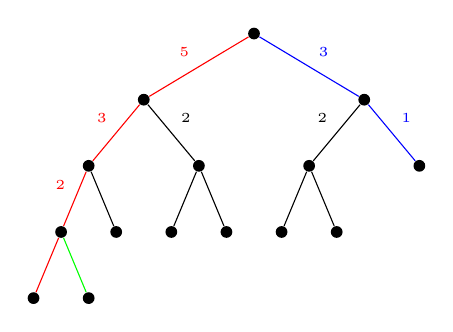
\begin{tikzpicture}[scale=0.7]

\node[circle, fill=black, inner sep=1.5pt] (root) at (0,0) {};
\node[circle, fill=black, inner sep=1.5pt] (n1) at (-2,-1.2) {};
\node[circle, fill=black, inner sep=1.5pt] (n2) at (2,-1.2) {};
\node[circle, fill=black, inner sep=1.5pt] (n3) at (-3,-2.4) {};
\node[circle, fill=black, inner sep=1.5pt] (n4) at (-1,-2.4) {};
\node[circle, fill=black, inner sep=1.5pt] (n5) at (1,-2.4) {};
\node[circle, fill=black, inner sep=1.5pt] (n6) at (3,-2.4) {};
\node[circle, fill=black, inner sep=1.5pt] (n7) at (-3.5,-3.6) {};
\node[circle, fill=black, inner sep=1.5pt] (n8) at (-2.5,-3.6) {};
\node[circle, fill=black, inner sep=1.5pt] (n9) at (-1.5,-3.6) {};
\node[circle, fill=black, inner sep=1.5pt] (n10) at (-0.5,-3.6) {};
\node[circle, fill=black, inner sep=1.5pt] (n11) at (0.5,-3.6) {};
\node[circle, fill=black, inner sep=1.5pt] (n12) at (1.5,-3.6) {};

% added nodes
\node[circle, fill=black, inner sep=1.5pt] (n13) at (-4,-4.8) {};
\node[circle, fill=black, inner sep=1.5pt] (n14) at (-3,-4.8) {};

% edges
\draw[red] (root) -- (n1) node[midway, above left] {\tiny $5$};
\draw[blue] (root) -- (n2) node[midway, above right] {\tiny $3$};
\draw[red] (n1) -- (n3) node[midway, above left] {\tiny $3$};
\draw (n1) -- (n4) node[midway, above right] {\tiny 2};
\draw (n2) -- (n5) node[midway, above left] {\tiny $2$};
\draw[blue] (n2) -- (n6) node[midway, above right] {\tiny 1};
\draw[red] (n3) -- (n7) node[midway, above left] {\tiny $2$};
\draw (n3) -- (n8);
\draw (n4) -- (n9);
\draw (n4) -- (n10);
\draw (n5) -- (n11);
\draw (n5) -- (n12);
\draw[red] (n7) -- (n13);
\draw[green] (n7) -- (n14);

\end{tikzpicture}
\end{minipage}
\hfill
\begin{minipage}{0.48\textwidth}
\centering
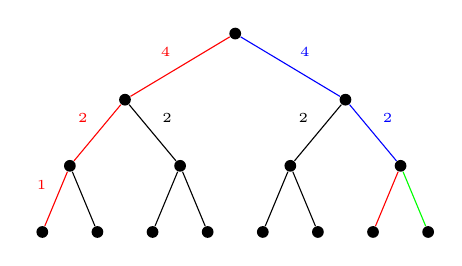
\begin{tikzpicture}[scale=0.7]

% Copy the same node layout for now; you can modify for T' later
\node[circle, fill=black, inner sep=1.5pt] (root) at (0,0) {};
\node[circle, fill=black, inner sep=1.5pt] (n1) at (-2,-1.2) {};
\node[circle, fill=black, inner sep=1.5pt] (n2) at (2,-1.2) {};
\node[circle, fill=black, inner sep=1.5pt] (n3) at (-3,-2.4) {};
\node[circle, fill=black, inner sep=1.5pt] (n4) at (-1,-2.4) {};
\node[circle, fill=black, inner sep=1.5pt] (n5) at (1,-2.4) {};
\node[circle, fill=black, inner sep=1.5pt] (n6) at (3,-2.4) {};
\node[circle, fill=black, inner sep=1.5pt] (n7) at (-3.5,-3.6) {};
\node[circle, fill=black, inner sep=1.5pt] (n8) at (-2.5,-3.6) {};
\node[circle, fill=black, inner sep=1.5pt] (n9) at (-1.5,-3.6) {};
\node[circle, fill=black, inner sep=1.5pt] (n10) at (-0.5,-3.6) {};
\node[circle, fill=black, inner sep=1.5pt] (n11) at (0.5,-3.6) {};
\node[circle, fill=black, inner sep=1.5pt] (n12) at (1.5,-3.6) {};

% reattached cherry
\node[circle, fill=black, inner sep=1.5pt] (n13) at (3.5,-3.6) {};
\node[circle, fill=black, inner sep=1.5pt] (n14) at (2.5,-3.6) {};


% edges
\draw[red] (root) -- (n1) node[midway, above left] {\tiny $4$};
\draw[blue] (root) -- (n2) node[midway, above right] {\tiny $4$};
\draw[red] (n1) -- (n3) node[midway, above left] {\tiny $2$};
\draw (n1) -- (n4) node[midway, above right] {\tiny 2};
\draw (n2) -- (n5)node[midway, above left] {\tiny 2};
\draw[blue] (n2) -- (n6) node[midway, above right] {\tiny $2$};
\draw[red] (n3) -- (n7) node[midway, above left] {\tiny $1$};
\draw (n3) -- (n8);
\draw (n4) -- (n9);
\draw (n4) -- (n10);
\draw (n5) -- (n11);
\draw (n5) -- (n12);
\draw[green] (n6) -- (n13);
\draw[red] (n6) -- (n14);

\end{tikzpicture}
\end{minipage}

\caption{Side-by-side illustration of the initial tree $T$ (left) and the tree $T'$ after balancing (right). The pruning path $\{e_i^p\}$ in red and the attachment path $\{e_i^a\}$ in blue are highlighted}
\label{fig:balancing_algorithm_trees}
\end{figure}
% endfig


Suppose that $\{\alpha_i\}_{i=1}^{2k-2}, \{\alpha_i'\}_{i=1}^{2k-2}$ are the descendant counts of $T, T'$ respectively. We claim that $\sum f(\alpha_i') \leq \sum f(\alpha_i)$, namely that this balancing operation can only decrease the overall sum. To see why, let
%
\[v = u_0 \xrightarrow{e^p_1} ... \xrightarrow{e^p_n} u_n = \ell_p, \quad v = w_0 \xrightarrow{e^a_1} ... \xrightarrow{e^a_m} w_m = \ell_a\]
%
\noindent be the paths we traverse the tree in our pruning (from $v \to \ell_p$) and grafting (from $v \to \ell_a$) operations respectively. Note that $\alpha_e = \alpha'_e$ for all edges $e \notin \{e_i^p\} \cup \{e_i^a\}$ not along either of these paths. Moreover, every edge along the pruning path loses exactly one descendant leaf and every edge along the attachment path gains exactly one leaf.  The edges in $T,T'$ are exactly the same, except for the relocation of the cherry, and hence we pair the descendant counts $\alpha_e, \alpha'_e$

\[\sum_i (f(\alpha_i) - f(\alpha'_i))=  \sum_{i=1}^{n-1} [f(\alpha_{e_i^p}) -  f(\alpha_{e_i^p} - 1)] + \sum_{i=1}^{m-1} [f(\alpha_{e_i^a}) -  f(\alpha_{e_i^a} + 1)].\]

\noindent Moreover,  by construction $m \leq n$ and $\alpha_{e_i^p} > \alpha_{e_i^a}$. This is because we always choose the larger subtree for pruning and the smaller for attaching. Thus $\alpha_{e_1^p} > \alpha_{e_1^a}$ and hence by induction
%
\[\alpha_{e_i}^p \geq \bigg\lceil \frac{\alpha_{e_{i-1}^p}}{2} \bigg \rceil > \bigg\lfloor \frac{\alpha_{e_{i-1}^a}}{2} \bigg \rfloor \geq \alpha_{e_i^a}\]
%
\noindent so $\alpha_{e_i^p} > \alpha_{e_i^a}$ is true for all $i$. Using this, we can see

\[= \sum_{i=1}^{m-1} [f(\alpha_{e_i^p}) -  f(\alpha_{e_i^p} - 1)] + [f(\alpha_{e_i^a}) -  f(\alpha_{e_i^a} + 1)] + \sum_{i=m}^{n-1} [f(\alpha_{e_i^p}) -  f(\alpha_{e_i^p} - 1)].\]

\noindent Each term in the first summand is nonnegative as $f$ is convex, and each term in the second summand is nonnegative as $f$ is increasing. Hence $\sum (f(\alpha_i) - f(\alpha_i')) \geq 0$ and the result follows.


Lastly, we argue that any tree can be converted into a balanced tree by iterating this procedure. If the subtrees of a given unbalanced vertex have size $L,R$ respectively where $L-R \geq 2$ then clearly after this procedure they have sizes $L-1, R+1$ respectively with imbalance $(L-1) - (R+1) = (L-R) - 2$. Hence the imbalance decreases by two, and if we iterate this procedure enough times we can get the imbalance to be $(L-R) \; mod(2)$, namely the vertex is balanced. Moreover, the descendant counts of any vertices not contained in one of the subtrees of $v$ are left unchanged. Hence we can start at the root and iteratively apply the procedure until the root is balanced. Then we can work our way down the tree. 
\end{proof}

\end{document}
